%%%%%%%%%%%%%FIX EQUATION NUMBERING !!!


\chapter[Accelerating structures]{Accelerating structures}

\section[Accelerating structures]{Accelerating structures}

\subsection[Elements of electromagnetism]{Elements of electromagnetism}

\subsubsection{Maxwell's equations in a medium}

It's well known since the basic courses of physics that the electromagnetic waves follow the Maxwell's equations, that in a medium are

\begin{center}
\begin{tabular}{ l l r }
$\nabla . \vec{D} = \rho_{free}$			\hspace{10mm}				&	$\nabla . \vec{B} = 0	$	& \hspace{10mm} \multirow{2}{*}{(2.1)}\\
$\nabla \times \vec{E} = - \frac{\partial \vec{B}}{\partial t}$		&	$\nabla \times \vec{H} = \vec{J}_{cond} + \frac{\partial \vec{D}}{\partial t}	$ &\\
\end{tabular}
\end{center}
where $\vec{D} = \epsilon \vec{E}$, $\vec{B} = \mu \vec{H}$ and $\vec{E} = \sigma \vec{J}$ (the full derivation and further details on the notation are available in any book on classical electromagnetism, such as \cite{Botta:EM, Jackson:ClassEM}). The propagation in vacuum is described by the same equations and can be easily derived from the (2.1) with the choice of the appropriate constants.

\subsubsection{Confined propagation of EM waves}

In some particular cases the confined propagation of electromagnetic waves is possible, and realised using a metal waveguide to lead all the energy in a single direction. In this section some useful results on the propagation in a waveguide will be stressed. 

%%%%%bello ma non bellissimo

Using the set of equation (2.1) and asking that the electric field is normal to the surface to avoid power dissipation due to the Joule effect (so $\vec{E} \times \vec{n} = 0$), it can be derived the set of admitted solutions for the propagation of the EM waves. Among the solutions, the most important are the \textit{Transverse Magnetic} solutions (T.M.), where the axial component of the magnetic field is null, and the \textit{Transverse Electric} solutions (T.E.), which is the same for the electric field.




\subsubsection[Particle acceleration]{Particle acceleration}

\cite{Kilpatrick:slides}



\subsection[Periodic structures and synchronous acceleration]{Periodic structures and synchronous acceleration}

In order to deliver a  constant energy gain to a charged particle two conditions have to be met:

\begin{enumerate}
\item The electromagnetic wave has to have a non-zero component in the direction of the motion of the particle
\item The phase velocity of a wave have to be the same of the particle velocity, in order to keep the relative phase constant, and so the acceleration
\end{enumerate}
using some results of the theory of EM waves it is possible to derive that the former cannot be accomplished in the free space, but can be easily met in a cavity (e.g. a waveguide), and to satisfy the latter is not sufficient simply using a waveguide, but is necessary a particular geometry, typically periodic geometries are used for this purpose.







\cite{Botta:EM}




\subsection[Constant gradient vs constant impedance structures]{Constant gradient vs constant impedance structures}
Lorem ipsum dolor sit amet, consectetur adipiscing elit. Sed dui sem, aliquam id ultricies sit amet, fermentum at magna. Aenean vitae rhoncus leo. Fusce gravida consequat lacus, a porta risus bibendum semper. Morbi eget auctor velit. Pellentesque eu lacinia nisi. Maecenas sed orci eu erat porta imperdiet ac non dui. Pellentesque a odio ac quam euismod tempor. Nulla in dapibus mauris, a sodales ex. In imperdiet enim sed ornare sollicitudin. Pellentesque habitant morbi tristique senectus et netus et malesuada fames ac turpis egestas. Donec vehicula metus eu nisi ornare euismod. Proin at ex non ex iaculis porta.

\subsection[Beam effect on the accelerating structure]{Beam effect on the accelerating structure}
Lorem ipsum dolor sit amet, consectetur adipiscing elit. Sed dui sem, aliquam id ultricies sit amet, fermentum at magna. Aenean vitae rhoncus leo. Fusce gravida consequat lacus, a porta risus bibendum semper. Morbi eget auctor velit. Pellentesque eu lacinia nisi. Maecenas sed orci eu erat porta imperdiet ac non dui. Pellentesque a odio ac quam euismod tempor. Nulla in dapibus mauris, a sodales ex. In imperdiet enim sed ornare sollicitudin. Pellentesque habitant morbi tristique senectus et netus et malesuada fames ac turpis egestas. Donec vehicula metus eu nisi ornare euismod. Proin at ex non ex iaculis porta.



\subsection[TD26 structures for the Main Beam of CLIC]{TD26 structures for the Main Beam of CLIC}
Lorem ipsum dolor sit amet, consectetur adipiscing elit. Sed dui sem, aliquam id ultricies sit amet, fermentum at magna. Aenean vitae rhoncus leo. Fusce gravida consequat lacus, a porta risus bibendum semper. Morbi eget auctor velit. Pellentesque eu lacinia nisi. Maecenas sed orci eu erat porta imperdiet ac non dui. Pellentesque a odio ac quam euismod tempor. Nulla in dapibus mauris, a sodales ex. In imperdiet enim sed ornare sollicitudin. Pellentesque habitant morbi tristique senectus et netus et malesuada fames ac turpis egestas. Donec vehicula metus eu nisi ornare euismod. Proin at ex non ex iaculis porta.



\section[High power limits and scaling laws]{High power limits and scaling laws}

The limiting factors for room-temperature high-gradient accelerators have been identified as \textit{field emission} and \textit{RF breakdown}. The former is the emission of electrons in the form of the so called \textit{"Dark current"}, that subtracts RF power, causes radiation and can produce wakefields; the latter is a limiting factor to the operation of accelerators and can damage the structures.\cite{Wang:1997ip}

The understanding of these phenomena is particularly challenging and requires a mixture of notions of disciplines such as surface physics, metallurgy, fabrication processes, microwaves, beam dynamic and plasma physics. At the moment a satisfactory unified theory of the processes that take place during the breakdowns have not been found yet, then the improvement of the structures is achieved using some scaling laws for the high power limitations, that have been deducted from the experience and the experiments on the structures tested so far. 


\subsection[Field emission law]{Field emission law}

\subsubsection{Emission from flat clean surface}

The field emission law was theorised by Fowler and Nordheim in 1928 and rule the current emission from a metal with applied an intense electric field. The derivation was carried on calculating the tunnel probability of electrons of the conduction band through the perfectly flat and clean surface of a metal. \\The applied electric field modify the potential barrier, and the current density of emitted electrons can be derived as the following, giving the  \textit{Fowler-Nordheim equation} \cite{Fowler173}
\begin{equation}
J_F = \frac{ 1.54\times10^{-6} \times 10^{4.52\phi^{-0.5}} E^2}{  \phi } \, \text{exp} \left ( -\frac{6.53\times 10^9 \phi^{1.5}}{E} \right ) \quad [A.m^{-2}]  \label{FNlaw}
\end{equation}
where $\phi$ is the work function of the material and $E$ is the applied electric field.

\subsubsection{Enhanced field emission}

It's well known that almost any surface is never perfectly clean and flat, and also the fact that the asperities of the surface provoke an enhancement of the local electric field. This behaviour lead to the phenomenon known as \textit{Enhanced Field Emission} (EFE), which major contributors are:
\begin{itemize}
\item Surface imperfection due to imperfect machining
\item Metallic dust
\item Molten craters after breakdowns
\item Absorbed gas
\end{itemize} 
and some others. These effects can create particular sites known as "emitters". It's a common praxis define the field enhancement factor $\beta$ to relate the electric field to the microscopic one
\begin{equation}
E_{m} = \beta E
\end{equation}
and the $\beta$ factors can be calculated according to the emitter's geometry \cite{Rohrbach:190223} as exploited in figure \ref{tip_factors}.
Once the local field is known, using the formula \ref{FNlaw} calculate the current emitted from EFE by an emitter site of area A gives 
\begin{equation}
I_F = \frac{ 1.54\times10^{-6} \times 10^{4.52\phi^{-0.5}} A \beta^2 E^2}{  \phi } \, \text{exp} \left ( -\frac{6.53\times 10^9 \phi^{1.5}}{\beta E} \right ) \quad [A]  \label{If}
\end{equation}
where $\beta E$ is the local field, $\phi$ is the work function of the material and $A$ the area of the considered emitter.

 In the RF case the average current emitted is given by similar calculations, averaging the electric field on an RF period. The full calculation is stressed in \cite{Wang:1997ip}. 

Experimental evidence of the dark current emission have been detected by setups equipped with Faraday Cups, as in \cite{Wuensch:advaces}.

The emission of dark current seems to be a precursor of the breakdown  process, even if the relationship between the two processes has not been clarified so far.

\begin{figure}[h]
\centering

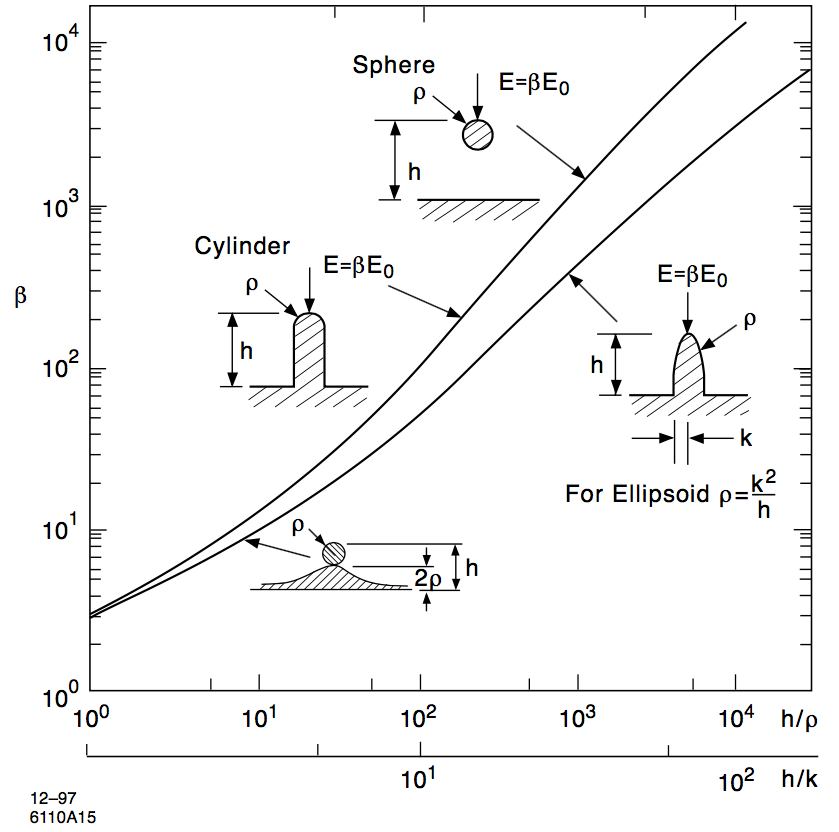
\includegraphics[scale=0.3]{pictures/beta_tip_val}
\caption{Field enhancement factors for simple geometries of metallic protrusions, plotted as function of geometrical features. From \cite{Rohrbach:190223}}
\label{tip_factors}

\end{figure}




\subsection[Kilpatrick's critereon]{Kilpatrick's critereon}

The Kilpatrick's Critereon was the first attempt to create a high power limit valid both in DC and RF applications \cite{KilpLimit}. The model was based on the acknowledgement of the Field Emission, and suggesting that the vacuum arc was created by the cascade of secondary electrons ejected from the surface by ion bombardment.

Using data collected in the 1950's, the following empirical law was formulated
\begin{equation}
W E^2 \text{exp} \left (  -1.7\times 10^5 E^{-1}  \right ) = 1.8 \times 10^{14}
\label{KilpLaw}
\end{equation}
where $W$ is the maximum possible ion energy in $eV$, and $E$ is the field in $V/m$.

\begin{figure}[h]
\centering

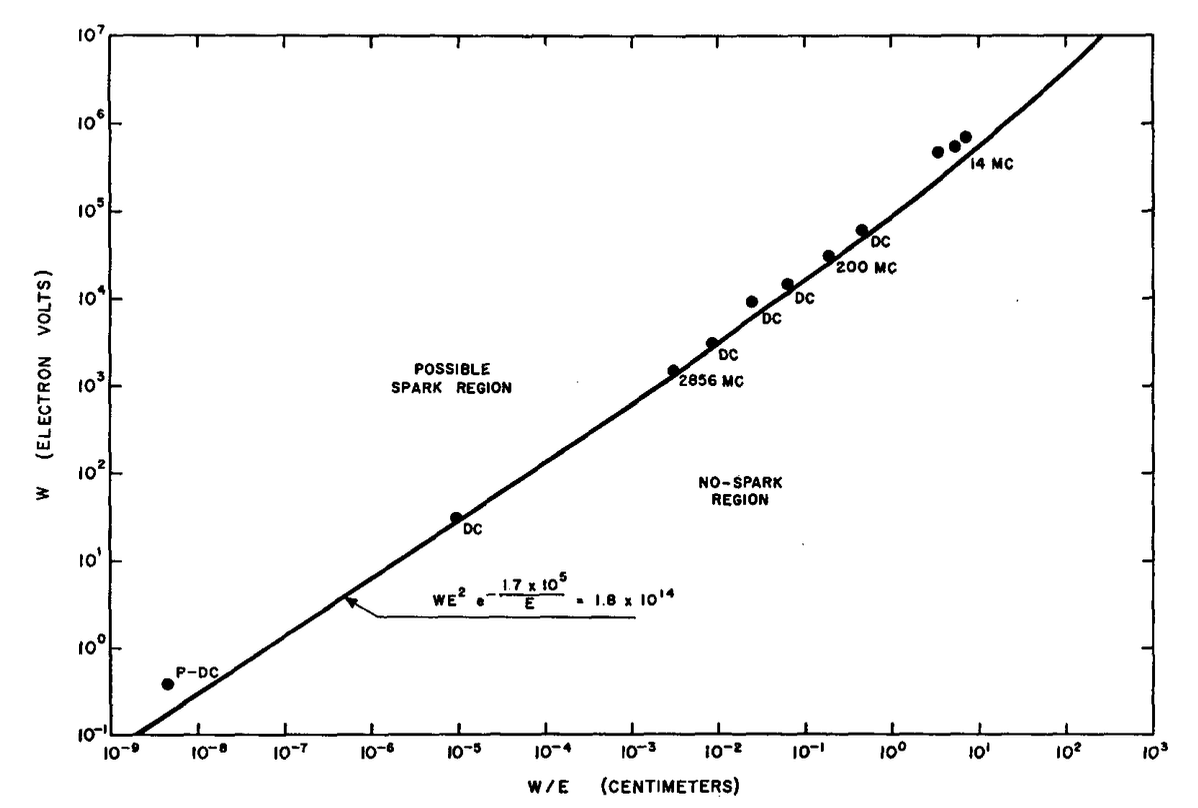
\includegraphics[scale=0.3]{pictures/kilpatrickCrit}
\caption{Kilpatrick's original plot, from \cite{KilpLimit}} $MC = MHz$ (\textit{Mega Cycles})
\label{kilpPlot}

\end{figure}

The critereon was reviewed many times up to now, because the experiments conducted nowadays show a limit up to 10 times lower than Kilpatrick's prediction, and this can be addressed to different reasons: first of all the quality of the machining of the structures have increased considerably since the 1950's; in second instance the formula for $W$ was deducted for parallel plates, but the condition inside the RF cavities are different during operations; and finally the key assumption was that the breakdown was triggered by the secondary emission provoked by the ion bombardment.

FREQUENCY DEPENDENCE ???
